%%%%%%%%%%%%%%%%%%%%%%%%%%%%%%%%%%%%%%%%%
% Focus Beamer Presentation
% LaTeX Template
% Version 1.0 (8/8/18)
%
% This template has been downloaded from:
% http://www.LaTeXTemplates.com
%
% Original author:
% Pasquale Africa (https://github.com/elauksap/focus-beamertheme) with modifications by 
% Vel (vel@LaTeXTemplates.com)
%
% Template license:
% GNU GPL v3.0 License
%
% Important note:
% The bibliography/references need to be compiled with bibtex.
%
%%%%%%%%%%%%%%%%%%%%%%%%%%%%%%%%%%%%%%%%%

%----------------------------------------------------------------------------------------
%	PACKAGES AND OTHER DOCUMENT CONFIGURATIONS
%----------------------------------------------------------------------------------------

\documentclass{beamer}

\usetheme{focus} % Use the Focus theme supplied with the template
% Add option [numbering=none] to disable the footer progress bar
% Add option [numbering=fullbar] to show the footer progress bar as always full with a slide count

% Uncomment to enable the ice-blue theme
\definecolor{main}{RGB}{92, 138, 168}
\definecolor{background}{RGB}{240, 247, 255}

%------------------------------------------------

\usepackage{booktabs} % Required for better table rules
\usepackage[utf8]{inputenc}
\usepackage[spanish]{babel}
\usepackage{enumitem}

%----------------------------------------------------------------------------------------
%	 TITLE SLIDE
%----------------------------------------------------------------------------------------

\title{Evaluación tecnológica de \\soluciones de gestión comercial para PYMES}

%\subtitle{Subtitle}

\author{Iman Hasnaouia Meskini\\ Álvaro Fernández Palma\\ Alina Altynguzhina \\ Cristina Díaz García}

\titlegraphic{\begin{flushright}
\includegraphics[scale=0.14]{imagenes/gestioncomercial.jpg}\end{flushright}} % Optional title page image, comment this line to remove it

%\institute{Institute Name \\ Institute Address}
\institute{Introducción a los Sistemas de Información}

\date{Octubre 2018}

%------------------------------------------------

\begin{document}

%------------------------------------------------

\begin{frame}
	\maketitle % Automatically created using the information in the commands above
\end{frame}

%----------------------------------------------------------------------------------------
%	 SECTION 1
%----------------------------------------------------------------------------------------

%\section{Quiénes somos} % Section title slide, unnumbered

%------------------------------------------------

\begin{frame}{Quiénes somos}

	Iman Hasnaouia Meskini
	
	Álvaro Fernández Palma
	
	Alina Altynguzhina
	
	Cristina Díaz García
	
\end{frame}

%------------------------------------------------

%\section{Introducción y objetivos} % Section title slide, unnumbered

%------------------------------------------------

\begin{frame}{Plan de trabajo}

\begin{enumerate}
	\item Divide y vencerás
	\item Deadlines
\end{enumerate}
	
\end{frame}

%------------------------------------------------

%\section{Tabla de datos} % Section title slide, unnumbered

%------------------------------------------------

\begin{frame}{Software propietario}

	\begin{center}
		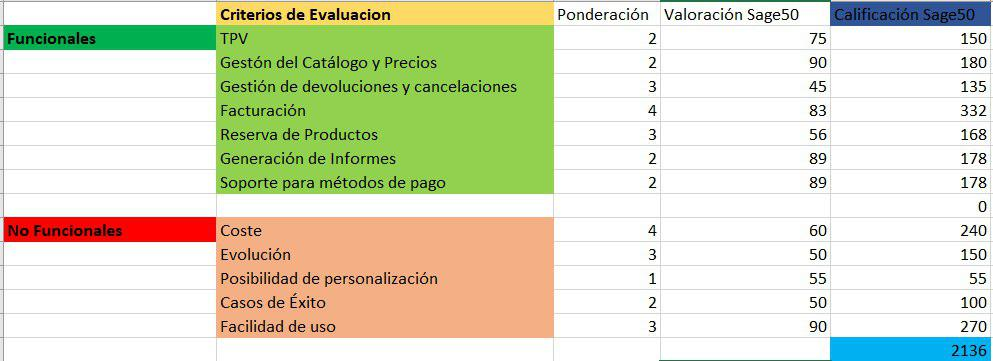
\includegraphics[scale=0.3]{imagenes/Sage50.jpg}
		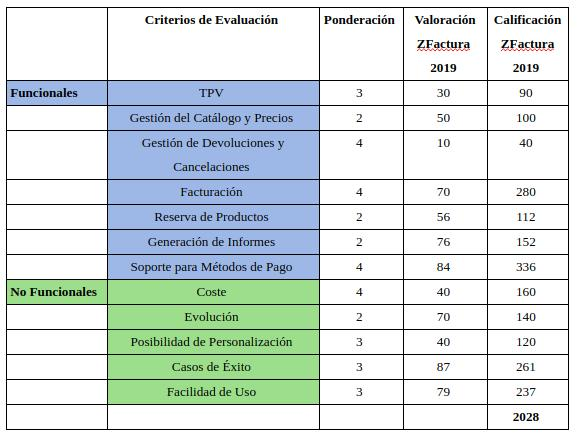
\includegraphics[scale=0.3]{imagenes/EvaluacionZFactura.jpg}
	\end{center}
	
\end{frame}

%------------------------------------------------

%\section{Indicadores} % Section title slide, unnumbered

%------------------------------------------------

\begin{frame}{Software Libre}

\begin{center}
	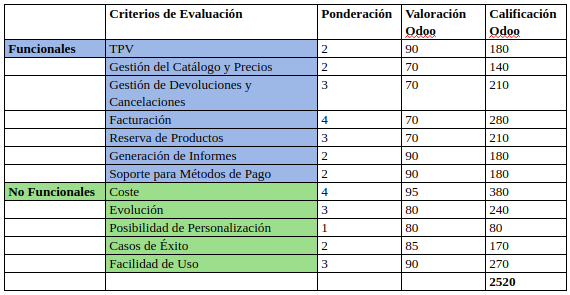
\includegraphics[scale=0.3]{imagenes/EvOdoo.png}
\end{center}
	
\end{frame}
	
%------------------------------------------------

%\section{Gráficos} % Section title slide, unnumbered

%------------------------------------------------

\begin{frame}{Software SaaS}

\begin{center}
	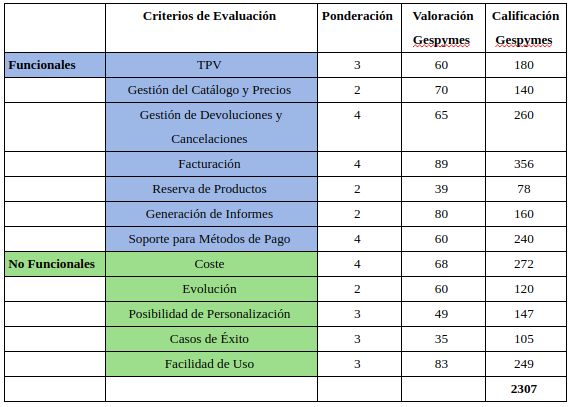
\includegraphics[scale=0.3]{imagenes/GespymesEv.png}
\end{center}
	
\end{frame}

\begin{frame}{Software SaaS}

\begin{center}
	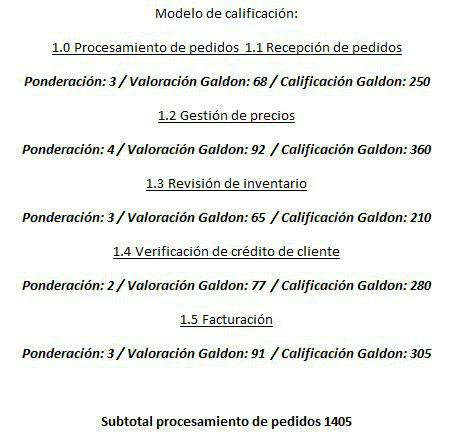
\includegraphics[scale=0.35]{imagenes/Galdon1.jpg}
	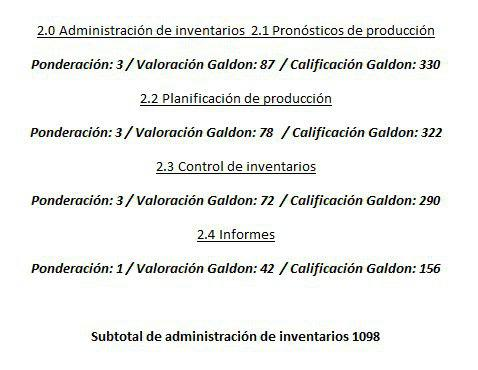
\includegraphics[scale=0.35]{imagenes/Galdon2.jpg}
	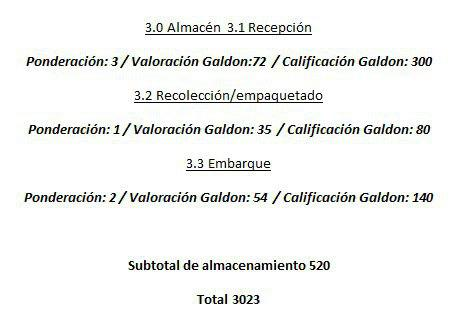
\includegraphics[scale=0.35]{imagenes/Galdon3.jpg}
\end{center}
	
\end{frame}

\begin{frame}{Software Movilidad}

\begin{center}
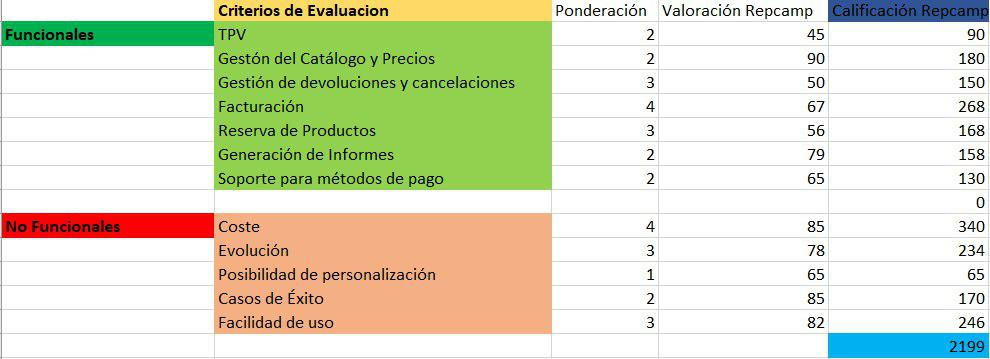
\includegraphics[scale=0.3]{imagenes/Repcamp.jpg} 
\end{center}
	
\end{frame}	

%------------------------------------------------

%\section{Conclusiones} % Section title slide, unnumbered

%------------------------------------------------

\begin{frame}{Conclusiones}

\begin{enumerate}
	\item Cada software estudiado, como todo, tiene unas ventajas y unas desventajas
	\item La elección del software dependerá de qué busquemos
	\item En nuestro caso, el elegido ha sido Galdon, un software de tipo SaaS
\end{enumerate}
	
\end{frame}
	
%------------------------------------------------

%\appendix
%
\begin{frame}{Bibliografía}
\begin{thebibliography}{9}

\bibitem{50Sage} \textit{50 Sage Cloud}, \url{https://www.sage.com/es-es/productos/sage-50-cloud/}.
\bibitem{CasosExito50Sage} \textit{Casos de éxito 50 Sage}, \url{http://partnews.sage.es/2018/01/caso-de-exito-sage-50c-con-office-365/}.
\bibitem{TPV50Sage} \textit{TPV 50 Sage}, \url{http://www.alcatic.com/sage-50-cloud/sage-50-cloud-tpv/}.
\bibitem{SaaSvsERP} \textit{Diferencias ERP tradicional y SaaS}, \url{https://www.gestionar-facil.com/software-de-gestion-erp-tradicional-vs-saas/}.
\bibitem{ERP} \textit{Definición ERP}, \url{https://www.galdon.com/erp-gestion-comercial-y-distribucion/}.
\bibitem{RepCamp} \textit{RepCamp}, \url{http://www.repcamp.com/es/index}.
\bibitem{RepCamp2} \textit{RepCamp}, \url{http://www.repcamp.com/es/plans}.
\bibitem{RepCamp3} \textit{RepCamp}, \url{http://www.repcamp.com/public/files/partners_es.pdf}.
\bibitem{TPVRepCamp} \textit{TPV en RepCamp}, \url{http://www.kriter.net/tecnologia-de-gestion-tpv}.
\bibitem{TPV2} \textit{Definición TPV}, \url{https://www.bbva.com/es/que-es-el-tpv/}.
\bibitem{CasosExitoRepCamp} \textit{Casos de éxito en RepCamp}, \url{http://www.kriter.net/images/files/PDF/Casos_exit/024_COMPARFARM.pdf}.
\bibitem{CasosExitoOdoo} \textit{Casos de éxito de Odoo}, \url{https://www.odoo.com/es_ES/page/cases}
\bibitem{FacturacionZFactura} \textit{Facturación ZFactura}, \url{https://www.ziclope.net/programas-de-facturacion/}
\bibitem{ZFactura} \textit{Videotutoriales ZFactura}, \url{https://www.ziclope.net/videotutoriales-zfactura/}
\bibitem{FacturaZFactura} \textit{Facturas ZFactura}, \url{https://www.modelofactura.net/programas/zfactura}
\bibitem{Gespymes} \textit{Gespymes}, \url{https://gespymes.es/}
\bibitem{DemoGespymes} \textit{Demos Gespymes}, \url{https://app.gespymes.es/licencias/demo_gespymes/index.php}
\end{thebibliography}
\end{frame}

%------------------------------------------------
%
%\begin{frame}{Backup Slide}
%	This is a backup slide, useful to include additional materials to answer questions from the audience.
%	\vfill
%	The package \texttt{appendixnumberbeamer} is used to refrain from numbering appendix slides.
%\end{frame}
%
%		COMMENTED SECTION
%		USEFUL TO GET SOME
%		INSPIRATION
%------------------------------------------------

%----------------------------------------------------------------------------------------
%
%\begin{frame}[plain]{Plain Slide}
%	This is a slide with the plain style and it is numbered.
%\end{frame}
%
%------------------------------------------------
%
%\begin{frame}[t]
%	This slide has an empty title and is aligned to top.
%\end{frame}
%
%------------------------------------------------
%
%\begin{frame}[noframenumbering]{No Slide Numbering}
%	This slide is not numbered and is citing reference \cite{knuth74}.
%\end{frame}
%
%------------------------------------------------
%
%\begin{frame}{Typesetting and Math}
%	The packages \texttt{inputenc} and \texttt{FiraSans}\footnote{\url{https://%fonts.google.com/specimen/Fira+Sans}}\textsuperscript{,}\footnote{\url{http://%mozilla.github.io/Fira/}} are used to properly set the main fonts.
%	\vfill
%	This theme provides styling commands to typeset \emph{emphasized}, \alert{alerted}, \%textbf{bold}, \textcolor{example}{example text}, \dots
%	\vfill
%	\texttt{FiraSans} also provides support for mathematical symbols:
%	\begin{equation*}
%		e^{i\pi} + 1 = 0.
%	\end{equation*}
%\end{frame}
%
%----------------------------------------------------------------------------------------
%	 SECTION 2
%----------------------------------------------------------------------------------------
%
%\section{Section 2}
%
%------------------------------------------------
%
%\begin{frame}{Blocks}
%	These blocks are part of 1 slide, to be displayed consecutively.
%	\begin{block}{Block}
%		Text.
%	\end{block}
%	\pause % Automatically creates a new "page" split between the above and above + below
%	\begin{alertblock}{Alert block}
%		Alert \alert{text}.
%	\end{alertblock}
%	\pause % Automatically creates a new "page" split between the above and above + below
%	\begin{exampleblock}{Example block}
%		Example \textcolor{example}{text}.
%	\end{exampleblock}
%\end{frame}
%
%%------------------------------------------------
%
%\begin{frame}{Columns}
%	\begin{columns}
%		\column{0.5\textwidth}
%			This text appears in the left column and wraps neatly with a margin between columns.
%		
%		\column{0.5\textwidth}
%			
\includegraphics[width=\linewidth]{Images/placeholder.jpg}
%	\end{columns}
%\end{frame}
%
%%------------------------------------------------
%
%\begin{frame}{Lists}
%	\begin{columns}[T, onlytextwidth] % T for top align, onlytextwidth to suppress the margin between columns
%		\column{0.33\textwidth}
%			Items:
%			\begin{itemize}
%				\item Item 1
%				\begin{itemize}
%					\item Subitem 1.1
%					\item Subitem 1.2
%				\end{itemize}
%				\item Item 2
%				\item Item 3
%			\end{itemize}
%		
%		\column{0.33\textwidth}
%			Enumerations:
%			\begin{enumerate}
%				\item First
%				\item Second
%				\begin{enumerate}
%					\item Sub-first
%					\item Sub-second
%				\end{enumerate}
%				\item Third
%			\end{enumerate}
%		
%		\column{0.33\textwidth}
%			Descriptions:
%			\begin{description}
%				\item[First] Yes.
%				\item[Second] No.
%			\end{description}
%	\end{columns}
%\end{frame}
%
%%------------------------------------------------
%
%\begin{frame}{Table}
%	\begin{table}
%		\centering % Centre the table on the slide
%		\begin{tabular}{l c}
%			\toprule
%			Discipline & Avg. Salary \\
%			\toprule
%			\textbf{Engineering} & \textbf{\$66,521} \\
%			Computer Sciences & \$60,005\\
%			Mathematics and Sciences & \$61,867\\
%			Business & \$56,720\\
%			Humanities \& Social Sciences & \$56,669\\
%			Agriculture and Natural Resources & \$53,565\\
%			Communications & \$51,448\\
%			\midrule
%			\textbf{Average for All Disciplines} & \textbf{\$58,114}\\
%			\bottomrule
%		\end{tabular}
%	\caption{Table caption}
%	\end{table}
%\end{frame}
%
%%------------------------------------------------
%
%\begin{frame}[focus]
%	Thanks for using \textbf{Focus}!
%\end{frame}
%
%%----------------------------------------------------------------------------------------
%%	 CLOSING/SUPPLEMENTARY SLIDES
%%----------------------------------------------------------------------------------------
%
%\appendix
%
%\begin{frame}{References}
%	\nocite{*} % Display all references regardless of if they were cited
%	\bibliography{example.bib}
%	\bibliographystyle{plain}
%\end{frame}
%
%%------------------------------------------------
%
%\begin{frame}{Backup Slide}
%	This is a backup slide, useful to include additional materials to answer questions from the audience.
%	\vfill
%	The package \texttt{appendixnumberbeamer} is used to refrain from numbering appendix slides.
%\end{frame}
%
%%----------------------------------------------------------------------------------------

\end{document}